\subsection{File}

\subsubsection{File size distribution}

\begin{figure}[!t]
	\centering
	\subfigure[CDF of files by file size (KB)]{\label{fig_cdf_file_size_kb}
		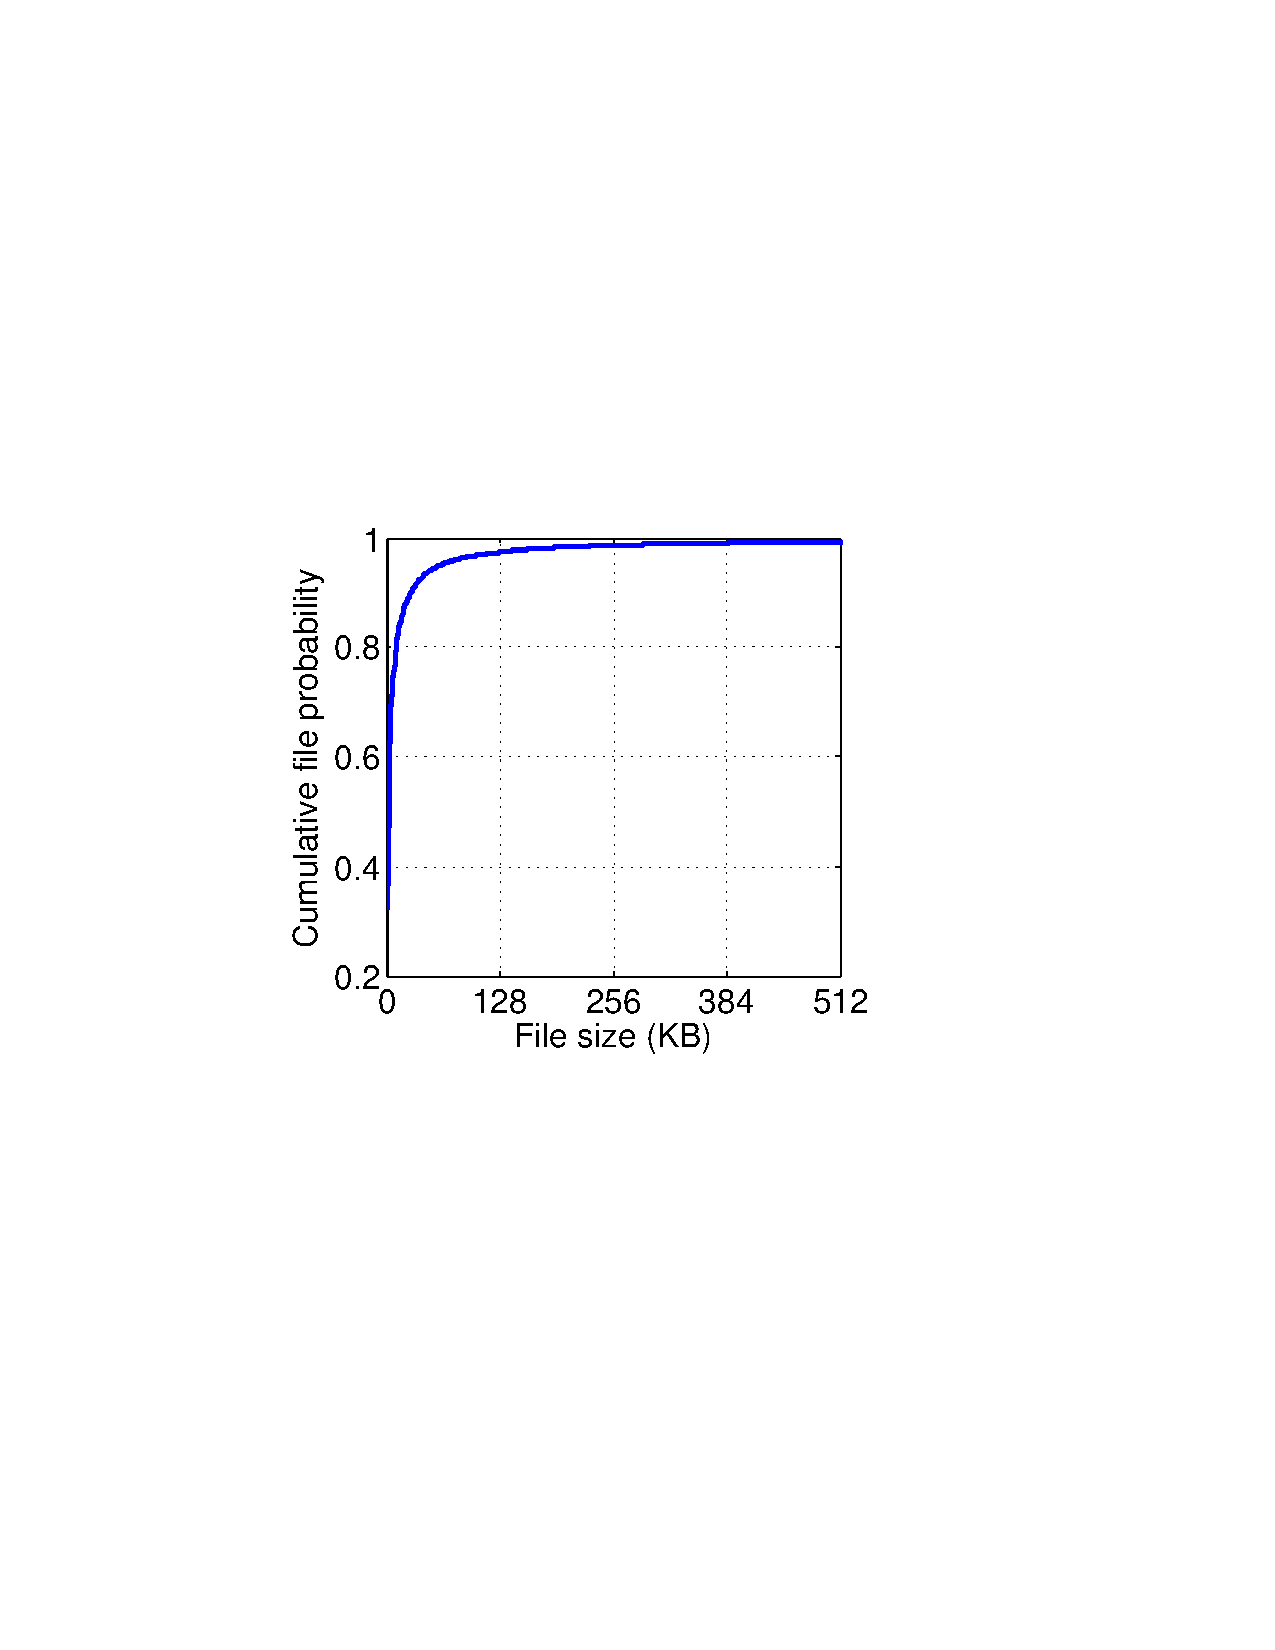
\includegraphics[width=0.23\textwidth]{graphs/cdf_file_size_kb.pdf}
	}
	\subfigure[Histogram of files by file size (KB)]{\label{fig_hist_file_size_kb}
		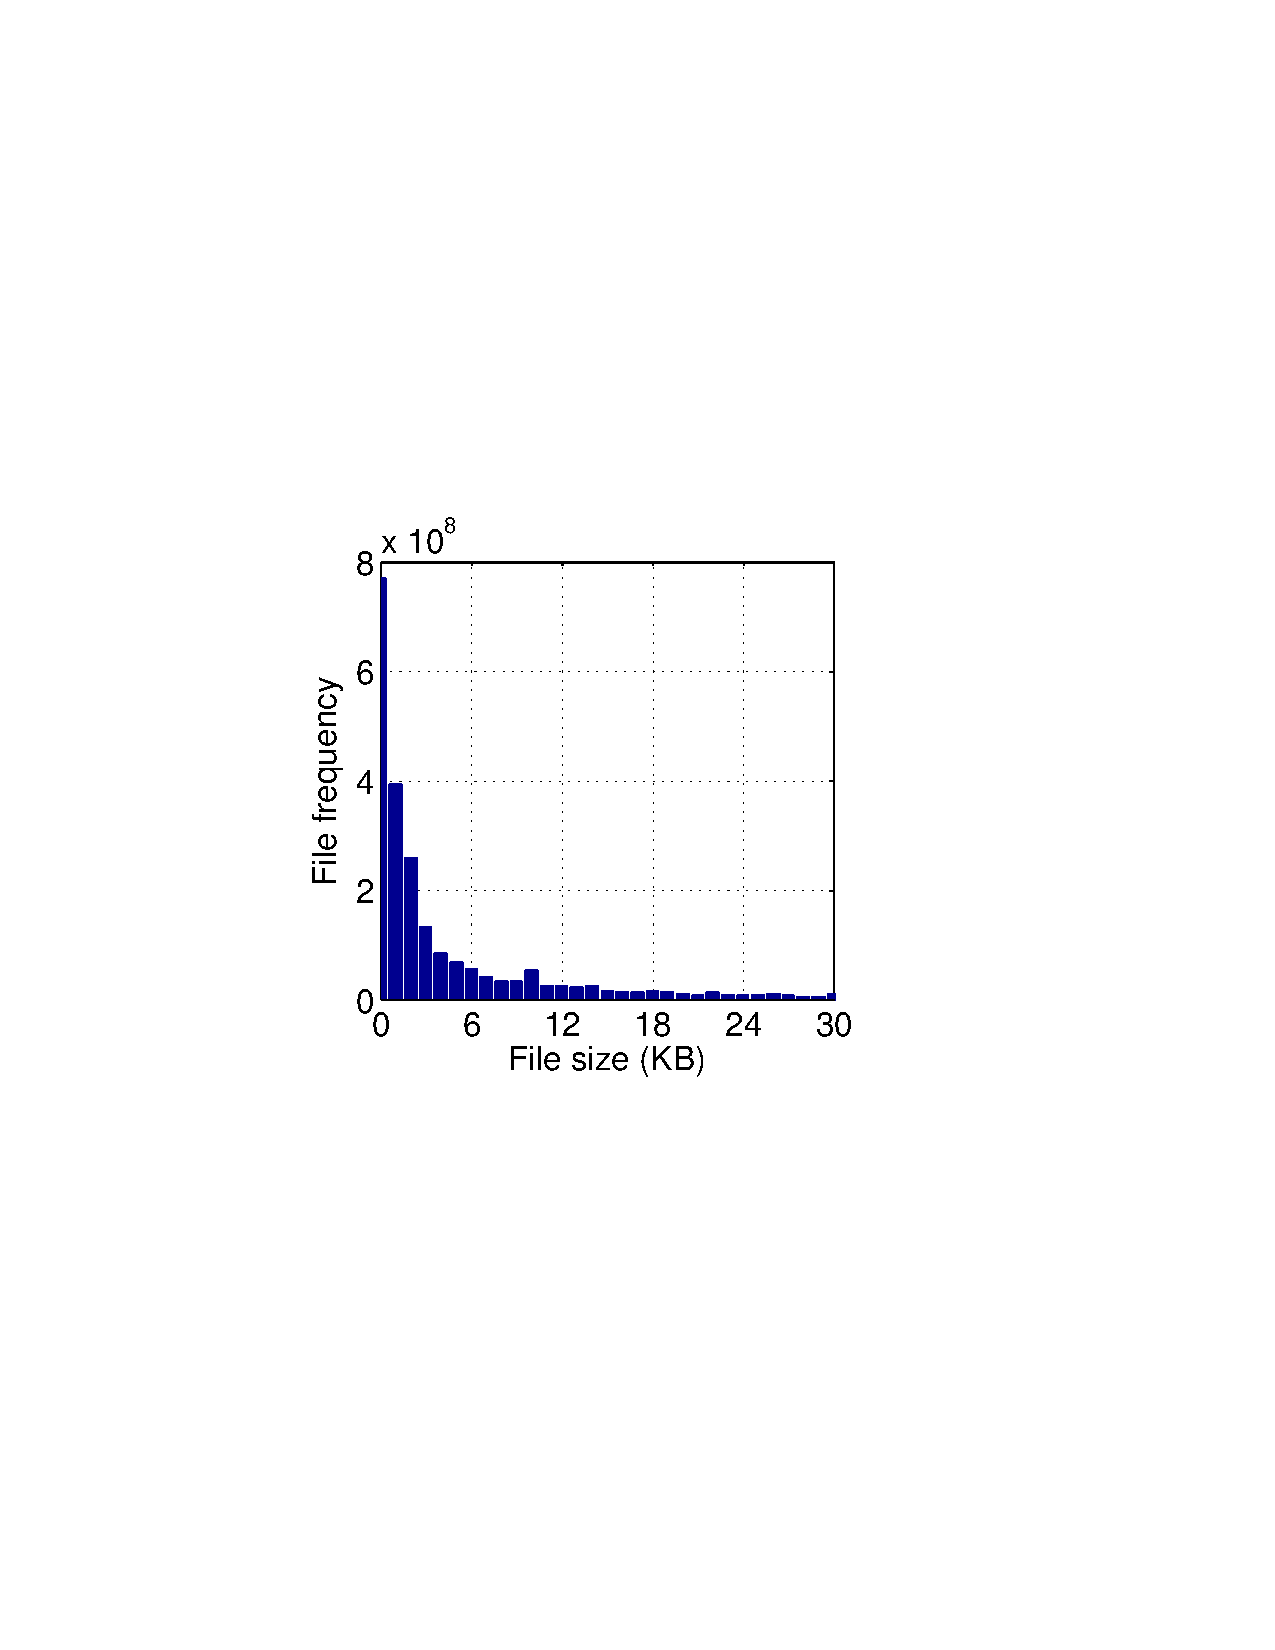
\includegraphics[width=0.22\textwidth]{graphs/hist_file_size_kb.pdf}
	}
	\caption{File size distribution}
	\label{fig-file-size}
\end{figure}

Figure~\ref{fig_cdf_file_size_kb} shows the cumulative file probability by file size. Around 90\% of files' sizes are less than 30 KB. 50\% of files' sizes are less than ~3. Figure~\ref{fig_hist_file_size_kb} shows the histogram of files by file size. About 769,000,000 files' sizes are less than 1 KB, which is the peak value in the figure. The maximum file size is ~12GB.

Figure~\ref{fig-file-size} suggests that majority of files in Docker images are small files. About 30\% of files are less than 1 KB. 99\% of files are smaller than 1 MB.

\subsubsection{File type distribution}

We use python library named python-magic~\cite{python-magic} to obtain the file type. Overall, there are 3,006,619,271 regular files and 282,379,663 symbolic links. Figure~\ref{fig-file-type} shows the top 22 file types. As shown, ASCII text is the most popular file type in Docker images. Around 886,843,570 (30\%) of files are ASCII text files. 
About 322,404,420 (11\%) files are gzip compressed files 
Interestingly, about 22,492,597 (1\%) of files are empty.  

\begin{figure*}
	\centering
	% Requires \usepackage{graphicx}
	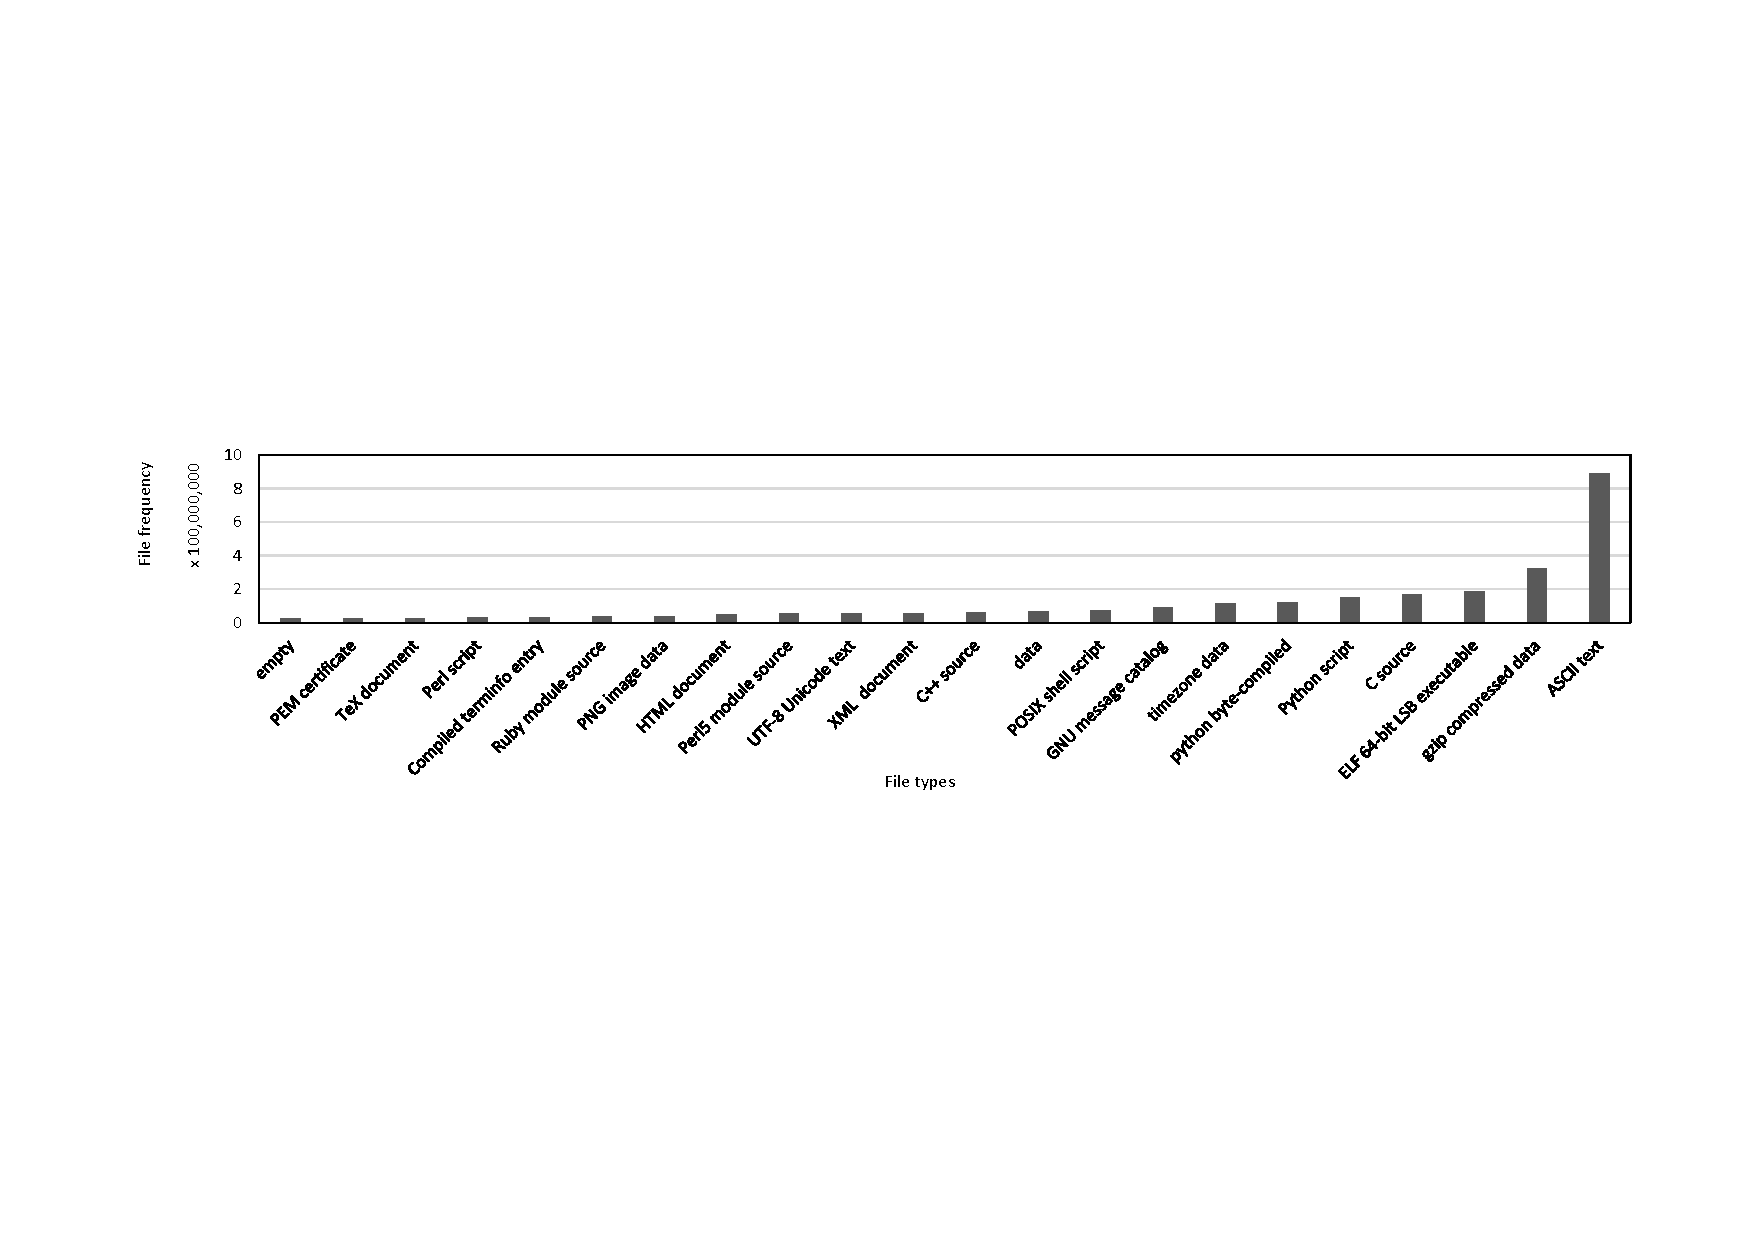
\includegraphics[width=1\textwidth]{graphs/file_type.pdf}\\
	\caption{File type distribution}\label{fig-file-type}
\end{figure*}
